% Use only LaTeX2e, calling the article.cls class and 12-point type.

\documentclass[12pt]{article}

% Users of the {thebibliography} environment or BibTeX should use the
% scicite.sty package, downloadable from *Science* at
% www.sciencemag.org/about/authors/prep/TeX_help/ .
% This package should properly format in-text
% reference calls and reference-list numbers.

\usepackage{scicite}
\usepackage{times}
\usepackage{graphicx}
\usepackage{lineno}
\usepackage{longtable}
%\usepackage{multicolumn}
\usepackage[skip=2pt,font=normalsize]{caption}
\usepackage[LGRgreek]{mathastext}
\usepackage{multirow}
\usepackage[
  breaklinks=true,
  colorlinks=true,
  linkcolor=blue,anchorcolor=blue,
  citecolor=blue,filecolor=blue,
  menucolor=blue,pagecolor=blue,
  urlcolor=blue]{hyperref}

% The following parameters seem to provide a reasonable page setup.

\topmargin 0.0cm
\oddsidemargin 0.2cm
\textwidth 16.5cm 
\textheight 21cm
\footskip 1.0cm


%The next command sets up an environment for the abstract to your paper.

\newenvironment{sciabstract}{%
\begin{quote} \bf}
{\end{quote}}

\usepackage{array}
\newcolumntype{L}[1]{>{\raggedright\let\newline\\\arraybackslash\hspace{0pt}}m{#1}}
\newcolumntype{C}[1]{>{\centering\let\newline\\\arraybackslash\hspace{0pt}}m{#1}}
\newcolumntype{R}[1]{>{\raggedleft\let\newline\\\arraybackslash\hspace{0pt}}m{#1}}

% If your reference list includes text notes as well as references,
% include the following line; otherwise, comment it out.

%\renewcommand\refname{References and Notes}

% The following lines set up an environment for the last note in the
% reference list, which commonly includes acknowledgments of funding,
% help, etc.  It's intended for users of BibTeX or the {thebibliography}
% environment.  Users who are hand-coding their references at the end
% using a list environment such as {enumerate} can simply add another
% item at the end, and it will be numbered automatically.

\newcounter{lastnote}
\newenvironment{scilastnote}{%
\setcounter{lastnote}{\value{enumiv}}%
\addtocounter{lastnote}{+1}%
\begin{list}%
{\arabic{lastnote}.}
{\setlength{\leftmargin}{.22in}}
{\setlength{\labelsep}{.5em}}}
{\end{list}}


% Include your paper's title here

%%%%%%%%%%%%%%%%% END OF PREAMBLE %%%%%%%%%%%%%%%%

\newcommand{\beginsupplement}{%
        \setcounter{table}{0}
        \renewcommand{\thetable}{S\arabic{table}}%
        \setcounter{figure}{0}
        \renewcommand{\thefigure}{S\arabic{figure}}%
     }


\begin{document} 
\beginsupplement

\linenumbers
\baselineskip24pt

\section*{Supplementary Information}% Make the title.

The following text provides additional information on this study's Methods and Results.  The full manuscript, data, and code for all calculations are available as part of an R package that can be installed from an accompanying \href{https://github.com/agroimpacts/ecoscales}{GitHub repository}.

\subsection*{Methods}% Make the title.

\vspace{-12pt}
%\begin{longtable}[h]
\begin{longtable}{lr}
%\centering
\caption{The selected journals and their 2012 impact factors.}\\
%\centering
%\begin{tabular}{lr}
  \hline
\textbf{Journal} & \textbf{Impact Factor} \\
\hline
\endhead 
  \hline
Ecology Letters & 17.95 \\ 
  Ecological Monographs & 8.09 \\ 
  Frontiers In Ecology And The Environment & 7.62 \\ 
  Global Ecology And Biogeography & 7.22 \\ 
  Global Change Biology & 6.91 \\ 
  Diversity And Distributions & 6.12 \\ 
  Methods In Ecology And Evolution & 5.92 \\ 
  Proceedings Of The Royal Society B-biological Sciences & 5.68 \\ 
  Journal Of Ecology & 5.43 \\ 
  Ecology & 5.17 \\ 
  Ecography & 5.12 \\ 
  Journal Of Biogeography & 4.86 \\ 
  Functional Ecology & 4.86 \\ 
  Journal Of Animal Ecology & 4.84 \\ 
  Journal Of Applied Ecology & 4.74 \\ 
  American Naturalist & 4.55 \\ 
  Conservation Biology & 4.36 \\ 
  Ecological Applications & 3.81 \\ 
  Biological Conservation & 3.79 \\ 
  Biogeosciences & 3.75 \\ 
  Bulletin Of The American Museum Of Natural History & 3.48 \\ 
  Biology Letters & 3.35 \\ 
  Oikos & 3.32 \\ 
  Behavioral Ecology & 3.22 \\ 
  Ecosystems & 3.17 \\ 
  Advances In Ecological Research & 3.08 \\ 
  Oecologia & 3.01 \\ 
  Landscape Ecology & 2.90 \\ 
  Agriculture Ecosystems \& Environment & 2.86 \\ 
  Ecological Economics & 2.85 \\ 
   \hline
%\end{tabular}
\label{tabs1}
\end{longtable}
% Place your abstract within the special {sciabstract} environment.

\subsubsection*{Scale FAQ}
\vspace{-10pt}
\noindent\underline{\textbf{General:}}
\def\Hitem{\item [Q\stepcounter{enumi}\arabic{enumi}.]} 
\def\Hsubitem{\item [Q\arabic{enumi}.\arabic{enumi}.]} 
\vspace{-0.5cm}
\begin{enumerate}
  \Hitem \emph{\textbf{What are the general inclusion/exclusion criteria for studies?}} Studies should be excluded from this analysis if they are: 1) opinion/perspectives pieces; 2) book reviews; 3) model-only studies, particularly theoretical models that are not developed or tested against observations; 4) if they are experimental manipulations (but if a study has a mix of observational and experimental treatments, record the former but exclude the latter).
  
  \Hitem \emph{\textbf{What are the standard categories to be used for defining observational method?}} Define observational method according to the following categories: Remote sensing or other geographic data (e.g. non-remotely sensed GIS data), passive/automated data collection, field/direct observation, or paleo-reconstruction (tree rings, charcoal cores, etc).

  \Hitem \emph{\textbf{What happens when the study draws on a separately published dataset as a key part of the methods?}} Track down the study describing the paper, and then record the DOI of that paper/those papers.
  
  \Hitem \emph{\textbf{What is the best unique identifier of a study I am reviewing?}} The DOI! 
  
  \Hitem \emph{\textbf{What do I record for a time or space scale when it is not clearly reported in the paper, or when I am unsure? For example, in a paleo-ecological study looking at historical charcoal deposition, sediment cores were extracted from lakes, which the authors report as the number of samples. However, it is unclear how many sediment cores were drawn from each lake, and it is these which should be the number of spatial replicates.}} For these sorts of issues, we record that the scale in question is uncertain, and then your best estimate of the measure (e.g. you might assume that only 1 core was made per lake).

\hspace{-1cm}\underline{\textbf{Temporal scales:}}
\vspace{-0.5cm} 
   \Hitem \emph{\textbf{What is interval, and how do we record it?}} Interval is the time that elapsed between repeated observations of the same point in space or individual organism. In many cases, observations will only be made one time--list a value of 0 for these.  
  \Hitem \emph{\textbf{What is sampling duration, and how do we record it?}} How long an individual observation of an individual point in space took to make. Sampling duration multiplied by the number of repeat observations is used to calculate \emph{actual duration} (see Q9). This value will often not be reported, so you will have to use your best judgement, based on your knowledge of ecological methods, to approximate the sampling duration. For example, for a field based method with intensive plot methods, if not enough information is provided to estimate a plausible sampling duration, assign a token 1 day. For remote sensing observations you can assume one second (although the observations are effectively instantaneous).  
   \Hitem \emph{\textbf{What is duration, and how do we estimate it?}} The duration is the total period of time over which the phenomenon of interest was observed. More specifically, in the case of repeated observations, this is the total time that elapsed between the first and last observations at a given point in space (or of the same individual organism or community). For once-off (unreplicated) observations, this time is equivalent to the sampling duration. However, there may be cases where once-off observations have a longer duration than the sample duration. For example, consider a study that counts occurrences of pollinators over three years, using transects that are located in different locations within the broader study area during each year \cite{rollin_differences_2013}. The observations are therefore not strictly temporally replicated, but the authors control for year of collection in their subsequent analysis to avoid confounding effects.  In this case, we can consider the effective duration to be three years, as the temporal information is encoded in the analysis. 
  \Hitem \emph{\textbf{What is \emph{actual duration}, and how do we calculate it?}} The actual duration is the integral of sampling duration (see Q7), or the time spent making one observation of the phenomenon in question. To clarify, actual duration is the total time spent sampling/observing a single point in space--not the span of time between first and last sample (duration), nor the integral of time spent in observing all spatial replicates (see Q10). 
  \Hitem \emph{\textbf{Should actual duration be the total time spent sampling all sites or the amount of time spent sampling per site (e.g. for 5 minute point counts of birds at 10 sites each repeated twice, should we enter 100 minutes (5 minutes X 2 repeats X 10 sites) or 10 minutes (5 minutes X 2 repeats) for duration)?}} As stated in Q9, actual duration is the total spent observing a single point in space, so in this case that would be 10 minutes (then converted to days, so 10 / (60 * 24))).
  \Hitem \emph{\textbf{How do we record duration and actual duration when there are no repeat observations?}} In these cases, duration and actual duration are both equal to sampling duration. 
   \Hitem \emph{\textbf{How do I record interval in cases where the interval is inconsistent?  For example, in a study where observations were repeated in 1979, 1980, 1981, 1984, 2007, 2009?}} Find the time between each successive period, and then take the average of that (remember to convert to days!). If there are two or more sets of unevenly spaced days for each site/plot/measurement being taken in the study, then find the average interval for each, and average the averages.  
    \Hitem \emph{\textbf{How do you determine the interval for paleo-reconstructions?}} Use the minimum estimate for dating precision as the estimate of time between samples (e.g. 50 years in the study of European charcoal deposits \cite{molinari_exploring_2013}). 
    \Hitem \emph{\textbf{How do you determine the sample duration (our third time category) for paleo-reconstructions?}} Similar to the answer to the previous question, the sampling duration is also the same as the minimum estimate of dating precision. The logic behind this is that in such cases, where a sediment or tree core or similar measurement is being collected, this effectively represents a continuous ``observation'', and the value associated with the minimum (or other reported) interval is typically an average (or another summary statistic like the maximum) of the amount accumulated. 
    \Hitem \emph{\textbf{What about intervals and durations for instrument-collected, or automated sensor-collected, observations?}} These are often similar to the paleo-reconstruction case. Take the minimum temperature or daily rainfall recorded at a weather station, which require constant observation over 24 hours to report. In such cases, the interval and sampling duration are both 24 hours. On the other hand, automated logging systems often provide a series of high frequency observations that are collected instantaneously. In these cases the sampling duration should be a token one second (to keep consistent with remote sensing [Q7]), and the interval should be the period between successive instantaneous measurements. 
    \Hitem \emph{\textbf{How do you treat interval for a case where repeated samples are taken during a season, across several seasons (e.g.``we performed repeat bird counts every 10 days between March and June of 2005, 2006, and 2008'')?}} Since the sampling is focused on seasons, and presumably interested in some season-dependent phenomenon (e.g. breeding behavior), the reported values should be pegged to the season, not averaged across the duration (the start and end dates of the study). So in this example it would be 10 days.  

\hspace{-1cm}\underline{\textbf{Spatial scales:}}
  \Hitem \emph{\textbf{What is resolution, and how do I record it?}} This is the finest scale at which a complete measurement of every unit of the quantity of interest is recorded.  For example, if the measurement in question is a tree stem count, the resolution is determined by the size of the plot used to record every tree stem. Taking this example further, let's say a study reports a plot size of 100 x 100 m, but then goes on to report that they counted stems within a single 1 m wide transect within this larger plot.  In this case, the plot resolution is in fact 100 m x 1 m, or 100 m$^2$ (sampling resolution should be reported in m$^2$).  In another example, if the reported plot size was 20 x 20 m, but the authors in fact only measured a random selection of, say, grass stems on which they counted aphids within those plots, then use an estimate of the area of the grass stem as the sampling resolution \cite{gagic_agricultural_2012}.  
 
  \Hitem \emph{\textbf{What is extent, and how do I record it?}} Extent is defined as the total area enclosed within a perimeter defined by the outermost spatial replicates, divided by 10,000 to convert to hectares. For studies in which spatial replicates are not spatially contiguous, this means the area of the minimum polygon bounding all spatial replicates. To calculate the effective survey extent, use the area of the study area/region given in the paper; when the area is not given, but when the survey region is given by name (e.g., Joshua Tree National Park or United States), look up the area through an online search and convert to hectares, provided the observations were collected throughout the named survey region. When the area is not named, but a map is given (or if the area is named and the map of replicates shows that the replicates were located in a smaller area of the named region), use an appropriate digitizing platform with a suitable map-providing backend (e.g. Google Earth Pro, QGIS with OpenLayers plugin) to navigate to the region and delineate a minimum convex polygon surrounding the replicates (plots/transects/other sampling units) to calculate the area in hectares. There is an exception to this rule, however, for studies that focus on features that are clearly distinct and functionally isolated from their surroundings. Examples of such cases might be mangrove forests patches within in a coastal National Park, or populations of a rare species confined to three disjunct protected areas. In these cases, the extent will be the summed area of the sampled units (the summed area of sampled mangrove stands, and the summed areas of the three protected areas). In other words, try to delineate the focal portions and not the larger survey region.
  
For spatially contiguous studies (e.g. those based on satellite imagery), the extent is the total area covered by the imagery (in such cases, extent equals actual extent), but only record the area of imagery analyzed by the authors (e.g. if the study area required four Landsat scenes to cover, but covered only the inner quarter of each image, report the extent as the summed area of the four quarters). However, if spatially contiguous studies only use a sub-sample of pixels, extent is the area of the polygon enclosing the outermost pixels (calculated following the methods above).

For studies that record individual, mobile organisms as the units of observation, use the minimum polygon surrounding the outermost observations of the complete space-time dataset (i.e. observations from all individuals and times) to define extent.

  \Hitem \emph{\textbf{What is \emph{actual extent}, and how do I record it?}}  Actual extent is the sampling resolution multiplied by the number of spatial replicates, divided by 10,000 to convert to hectares. For studies in which the spatial replicates are not spatially contiguous (as with most field-based studies), this means resolution (see Q17) multiplied by number of plots. For spatially contiguous studies (e.g., those based on remote sensing imagery), it should be the total area covered by the imagery, i.e., pixel resolution multiplied by the number of pixels. However, as with extent, only record the area analyzed by the authors. If they used a sub-sample of pixels, the actual extent is the number of those pixels multiplied by pixel resolution. 
  
    \Hitem \emph{\textbf{How do you determine resolution for paleo-reconstructions and other approaches where a sampling method is presumed to draw from a larger area (e.g. mammal traps, mist nets, etc)?}}  For sampling resolution, estimate the size of the sample actually taken, rather than the assumed catchment/shed area of the sample (e.g. the area of the corer used to take a sediment sample, rather than an estimate of the area that that sample is assumed to draw from), and then indicate that the plot resolution was uncertain. Related to this, you may also have to estimate the number of samples collected, as exemplified in a charcoal study of Europe where the number of lakes sampled was provided, not the number of cores per lake \cite{molinari_exploring_2013}.  

  \Hitem \emph{\textbf{What about studies that sample individual organisms?}} If the study is making a total count of all organisms (let's say a mammal species) within a fixed plot size, or even a variable plot size from which an average plot size (and thus sampling resolution) can be estimated, then follow the procedures described in Q17. However, if the individual animals are the unit of measure (either because a sub-sample of them is being made within a defined plot, or because the observation is not contingent on being located within a plot (maybe a blood sample or body weight is being recorded, for example), then simply estimate two-dimensional area occupied by the animal as the plot resolution, and the number of sampled animals provide the spatial replicates (for calculating actual extent). Occasionally individual animals might be recorded, but within the context of some natural feature, such as a nesting site where the survival of individual chicks is the measurement of interest \cite{roche_relative_2008}. In this case, an estimate of the nest area provides the sampling resolution. In cases where individual animals are tracked using radio or GPS collars, to calculate actual extent, use the number of locational fixes as the quantity of spatial replicates and the animal's two-dimensional body area. If the number of GPS points is not given, the number of fixes can be estimated from the duration during which individuals were collared and the recording interval.
\end{enumerate}

\subsection*{Results}
\vspace{-4pt}

\subsubsection*{Variability and consistency between observers}
\vspace{-10pt}

We assessed variability and consistency between observers along multiple dimensions. First, we assessed the degree to which observers agreed with respect to selecting or rejecting papers for review, using R's Agreement package \cite{yu_agreement:_2012} to calculate Fleiss' kappa statistic \cite{fleiss_measuring_1971}, which was 0.72 (z = 12.5, p$<$0.000), indicating substantial and significant agreement between observers \cite{landis_measurement_1977}. 

Second, we calculated the intra-class correlation coefficient \cite{bartko_intraclass_1966} to assess agreement between observers regarding the number of ecological observations that could be extracted from each paper (multiple ecological observations were reported in many studies; we listed observations as separate records if they measured different features, or more rarely, varied substantially on one or more dimensions).  The coefficient, calculated using the IRR package \cite{gamer_irr:_2012} of R, was 0.71 (F = 15.4, p$<$0.0001, 95\% confidence interval = 0.54 - 0.85)  

Finally, we calculated the coefficient of variation (CV) between observers' estimates of scales for each dimension, first across all observers' mean scale estimates, and then as the average CV among observers' estimates of each individual record (Table \ref{tabs2}). CV values were estimated from all six observers for resolution, actual extent, and interval, from five observers (all but Choi) for duration, and from three observers (Elsen, Estes, and Treuer) for extent. The smaller numbers for duration and extent reflect the fact that initial efforts were focused on estimating resolution, interval, and actual extent and actual duration. Fewer observers were available for subsequent efforts to assess duration and extent. 

\subsubsection*{Between-observer coefficient of variation}
\vspace{-10pt}
We used the maximum uncertainty values for each dimension from the inter-observer variability analysis (Table \ref{tabs2}) to determine the bounds of the random perturbations applied to each record over the 1000 iteration resample.  

\begin{table}[ht]
\captionsetup{width=1\linewidth}
\caption{The between-observer variability of estimates of the spatial and temporal scales of ecological observations reported within the set of 20 papers used for calibration. Variability is expressed as the coefficient of variation (CV; standard deviation divided by mean multiplied by 100) between each observer's overall mean, and as the mean CV of observers' estimates for individual records.}
\vspace{-4 pt}
\begin{center}
\begin{tabular}{rR{1.5cm}R{1.5cm}R{1.5cm}R{1.5cm}R{1.5cm}R{1.5cm}}
\hline
& \multicolumn{3}{c}{\textbf{Spatial}} & \multicolumn{3}{c}{\textbf{Temporal}}\\\cline{2-7}
%Value & Resolution & Extent & \multirow{2}{*}{Actual} & Interval & Duration & Actual Duration \\
Value & Resolution & Extent & Actual Extent & Interval & Duration & Actual Duration \\
\hline
CV of overall mean & 50 & 50 & 78 & 49 & 36 & 109 \\
Mean of record-wise CV & 58 & 41 & 72 & 105 & 64 & 126 \\
\hline
\end{tabular}
\end{center}
\label{tabs2}
\end{table}%

\subsubsection*{The domains of observational methods}
\vspace{-10pt}

Fig. \ref{obshists} details the distributions of observations separated by observational method along the four primary dimensions. Fig. \ref{obskde} shows the densities of observations by observational method within the dimensional juxtapositions shown in Fig. 2 in the main text. Fig. \ref{obsdiff} shows the how the differences between actual extent and extent and actual duration and duration vary by observational type.  

\subsubsection*{Trends in methods and scales}
\vspace{-10pt}
The results of the weighted linear regression applied to observational types by year (Fig. \ref{type_by_yr}) suggest an increase (by 1.3\% per year) in the use of remote sensing and a corresponding decline in field methods (by the same percentage) during the 2004-2014 time period, although neither trend is statistically significant (p$<$0.12 for regression of remote observations; p$<$0.18 for field observation regression).  Automated sensing methods showed no visible trend. 

If this trend towards increasing use of remote sensing between 2004-2014 was real and not spurious, we can project that a repeated study applied to papers published between 2004-2017 would find remote sensing used for 7.7\% of observations (a 22\% increase), which would increase mean extent by 17.4\% (95\% CI = -1.3-67\%;  or 0.07 orders of magnitude) above the 2004-2014 average. We cannot attach much confidence to this projections given that it derived from a non-significant trend; however, some support for this projection lies within the regression analysis applied to extent values themselves, which showed an apparent increase in extent of 0.25 orders of magnitude per year (Fig. \ref{sc_by_yr}) between 2004-2014 (R$^2$ = 0.25, p$<$0.07). This weak trend suggests that including more recent studies would have increased mean extent, but by a more modest 5.5\% (0.02 orders of magnitude).  The other three dimensions did not show any clear year-on-year trends. 

\subsubsection*{Choice of bandwidth in kernel density estimation}
\vspace{-10pt}
Figure \ref{ksens} indicates the effect that varying bandwidth has on the appearance of the kernel density estimates. The smallest bandwidth (0.4) tested (Fig. \ref{ksens} top) shows the same primary observational concentrations revealed in Fig. 1 in the main text, but these tend to be divided into separate sub-concentrations. An example is the oblong concentration of observations in Fig. 2A (and in the lower left panel in Fig. \ref{ksens}) that is bounded on the upper left at monthly to yearly intervals and 100-1000 m$^2$ resolutions, and on the lower right by near-daily to monthly observations and 0.1-10 ha resolutions. With the smaller bandwidth this concentration appears as two separate patches (Fig. \ref{ksens} top left), but with 0.7 bandwidth applied becomes coherent (Fig. \ref{ksens} middle left). It is expected that density clusters will increasingly separate as bandwidth is reduced. Nevertheless, this assessment indicates that the choice of bandwidth does not alter our primary interpretations, as the domains of highest and lowest concentrations remain the same regardless of bandwidth.  

\begin{figure}[!ht]
\centering
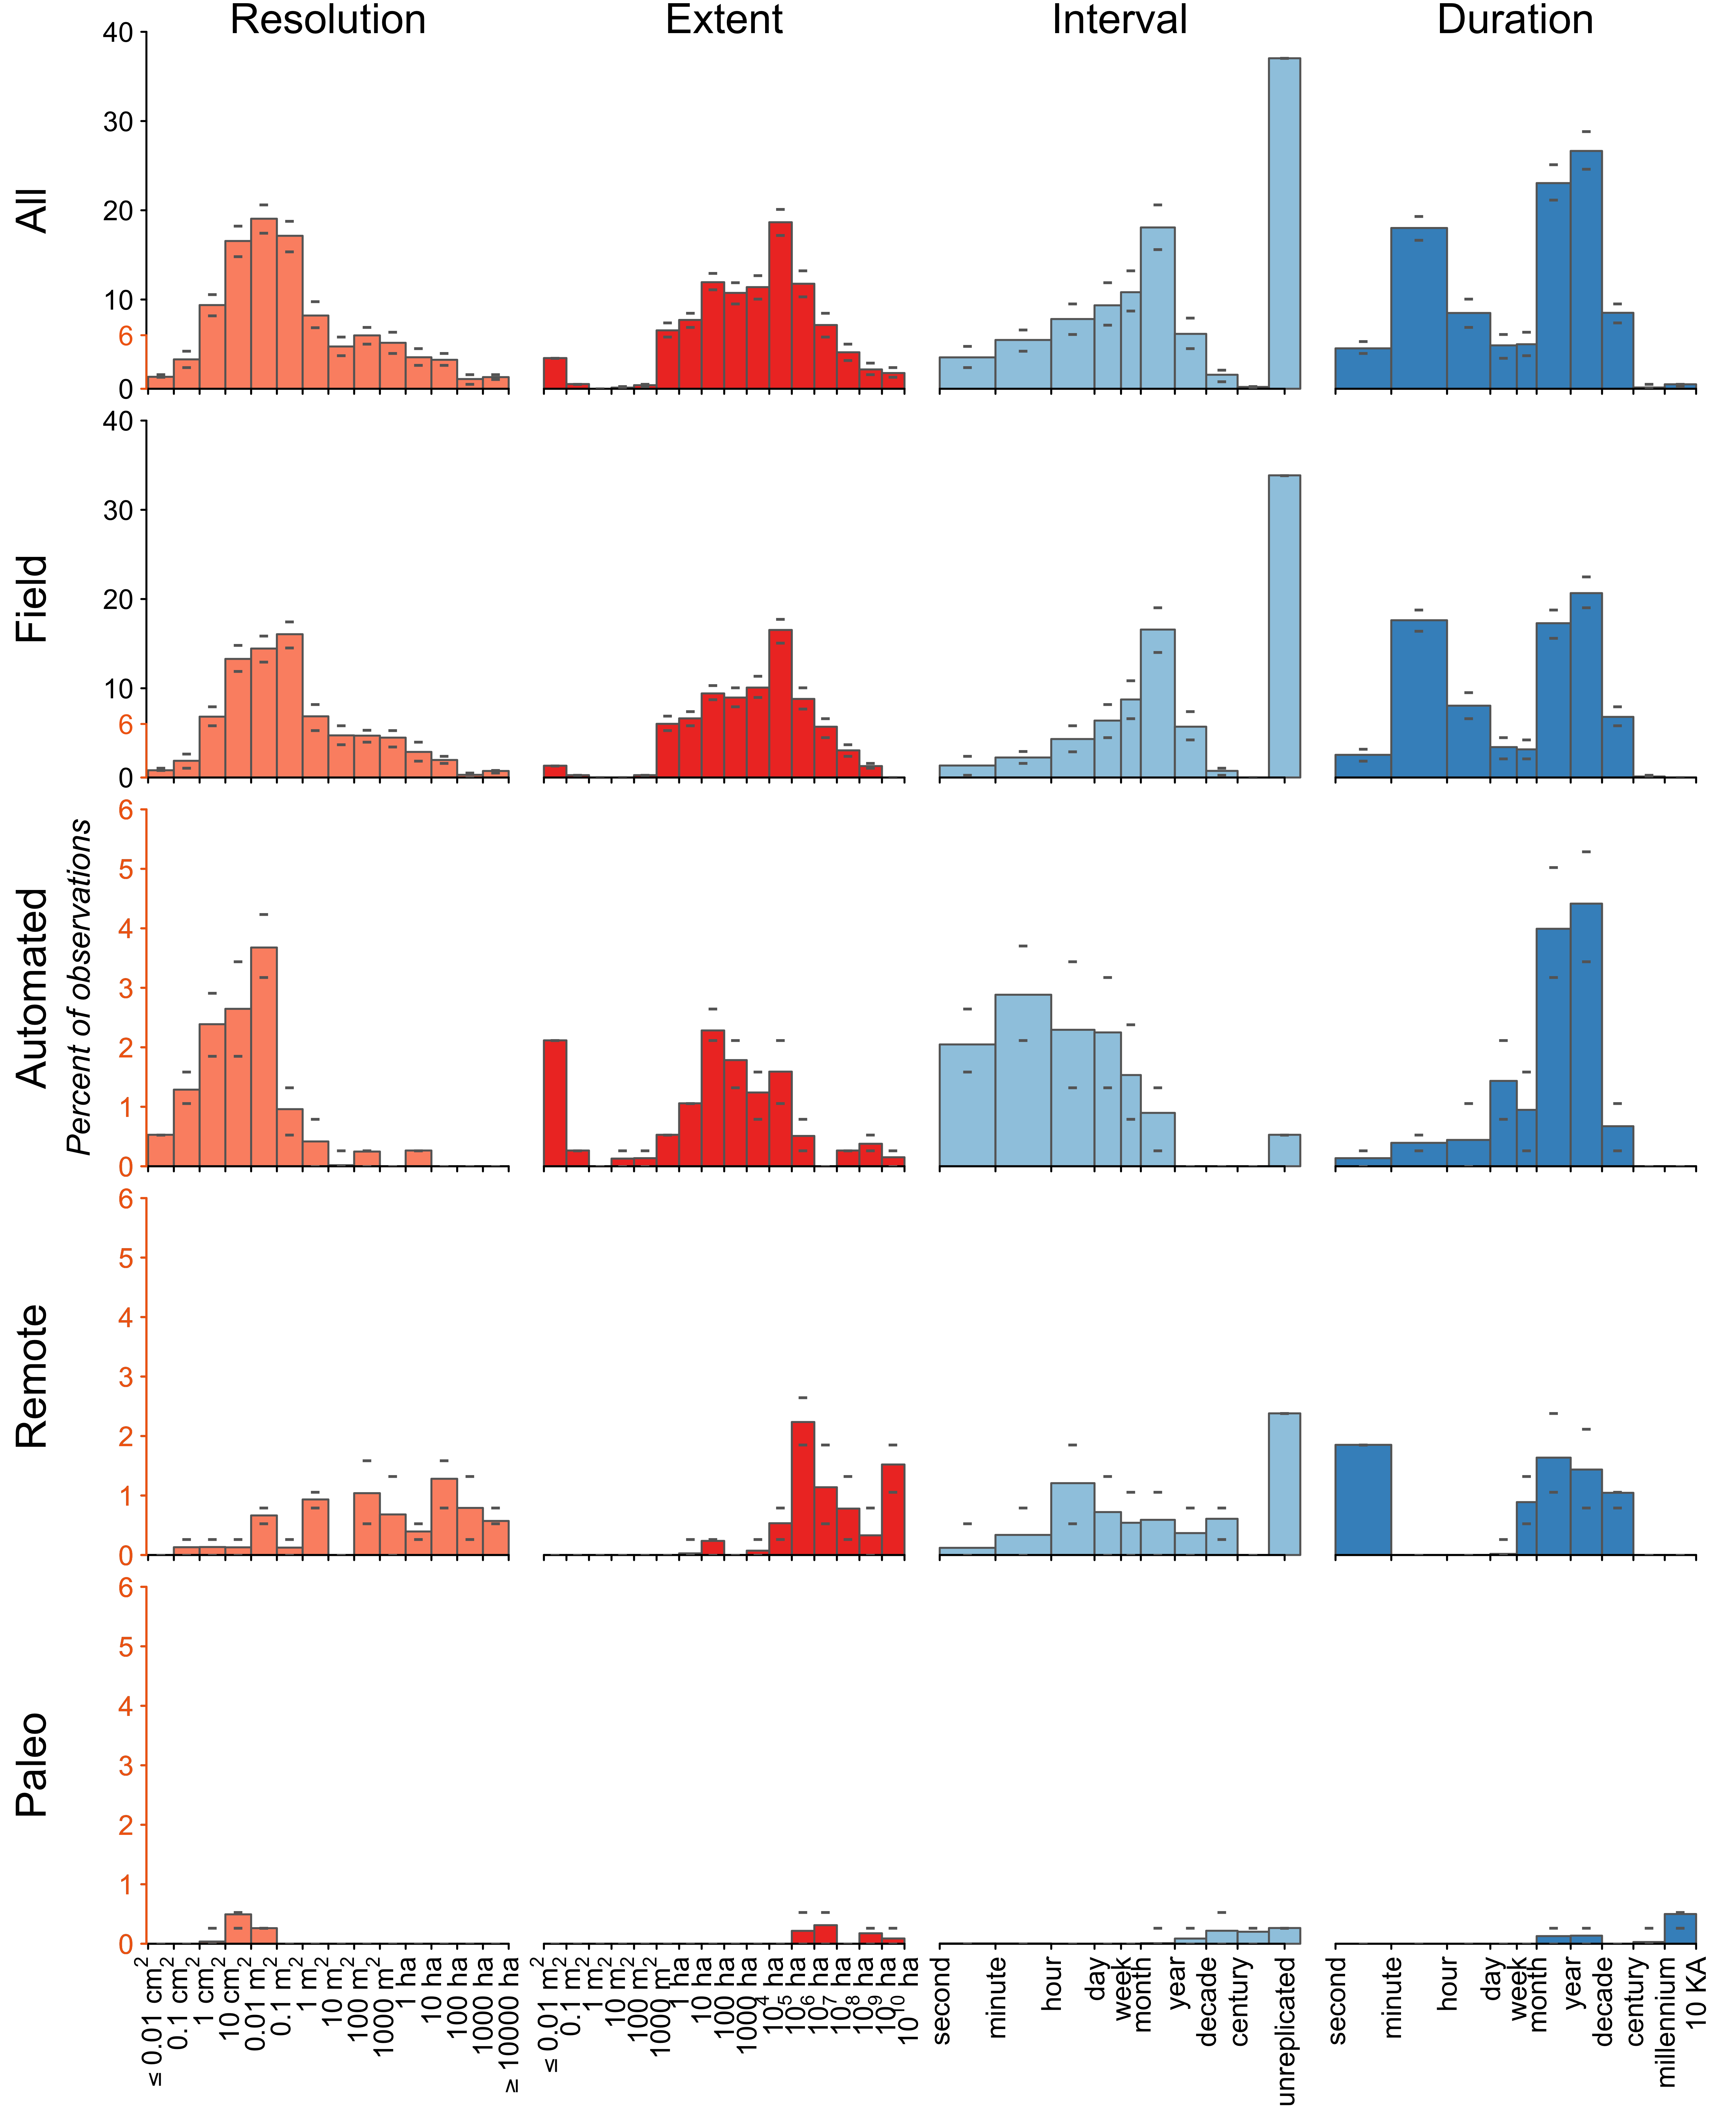
\includegraphics[width=0.9\textwidth]{../vignettes/figures/figS1.png}
\vspace{-5 pt}
\caption{Histograms of the resolution, extent, interval, and duration of observational scales, shown for all observational methods (top row) and for the four main observational methods (rows 2-5). Bars represent the average percentages for each bin realized after 1000 perturbed resamples, while grey bars indicate the 95\% confidence interval. Bar widths for interval and duration indicate differences in scale between x-axis labels. }
\label{obshists}
\end{figure}

\begin{figure}[!ht]
%\begin{wrapfigure}{c}{1\textwidth}
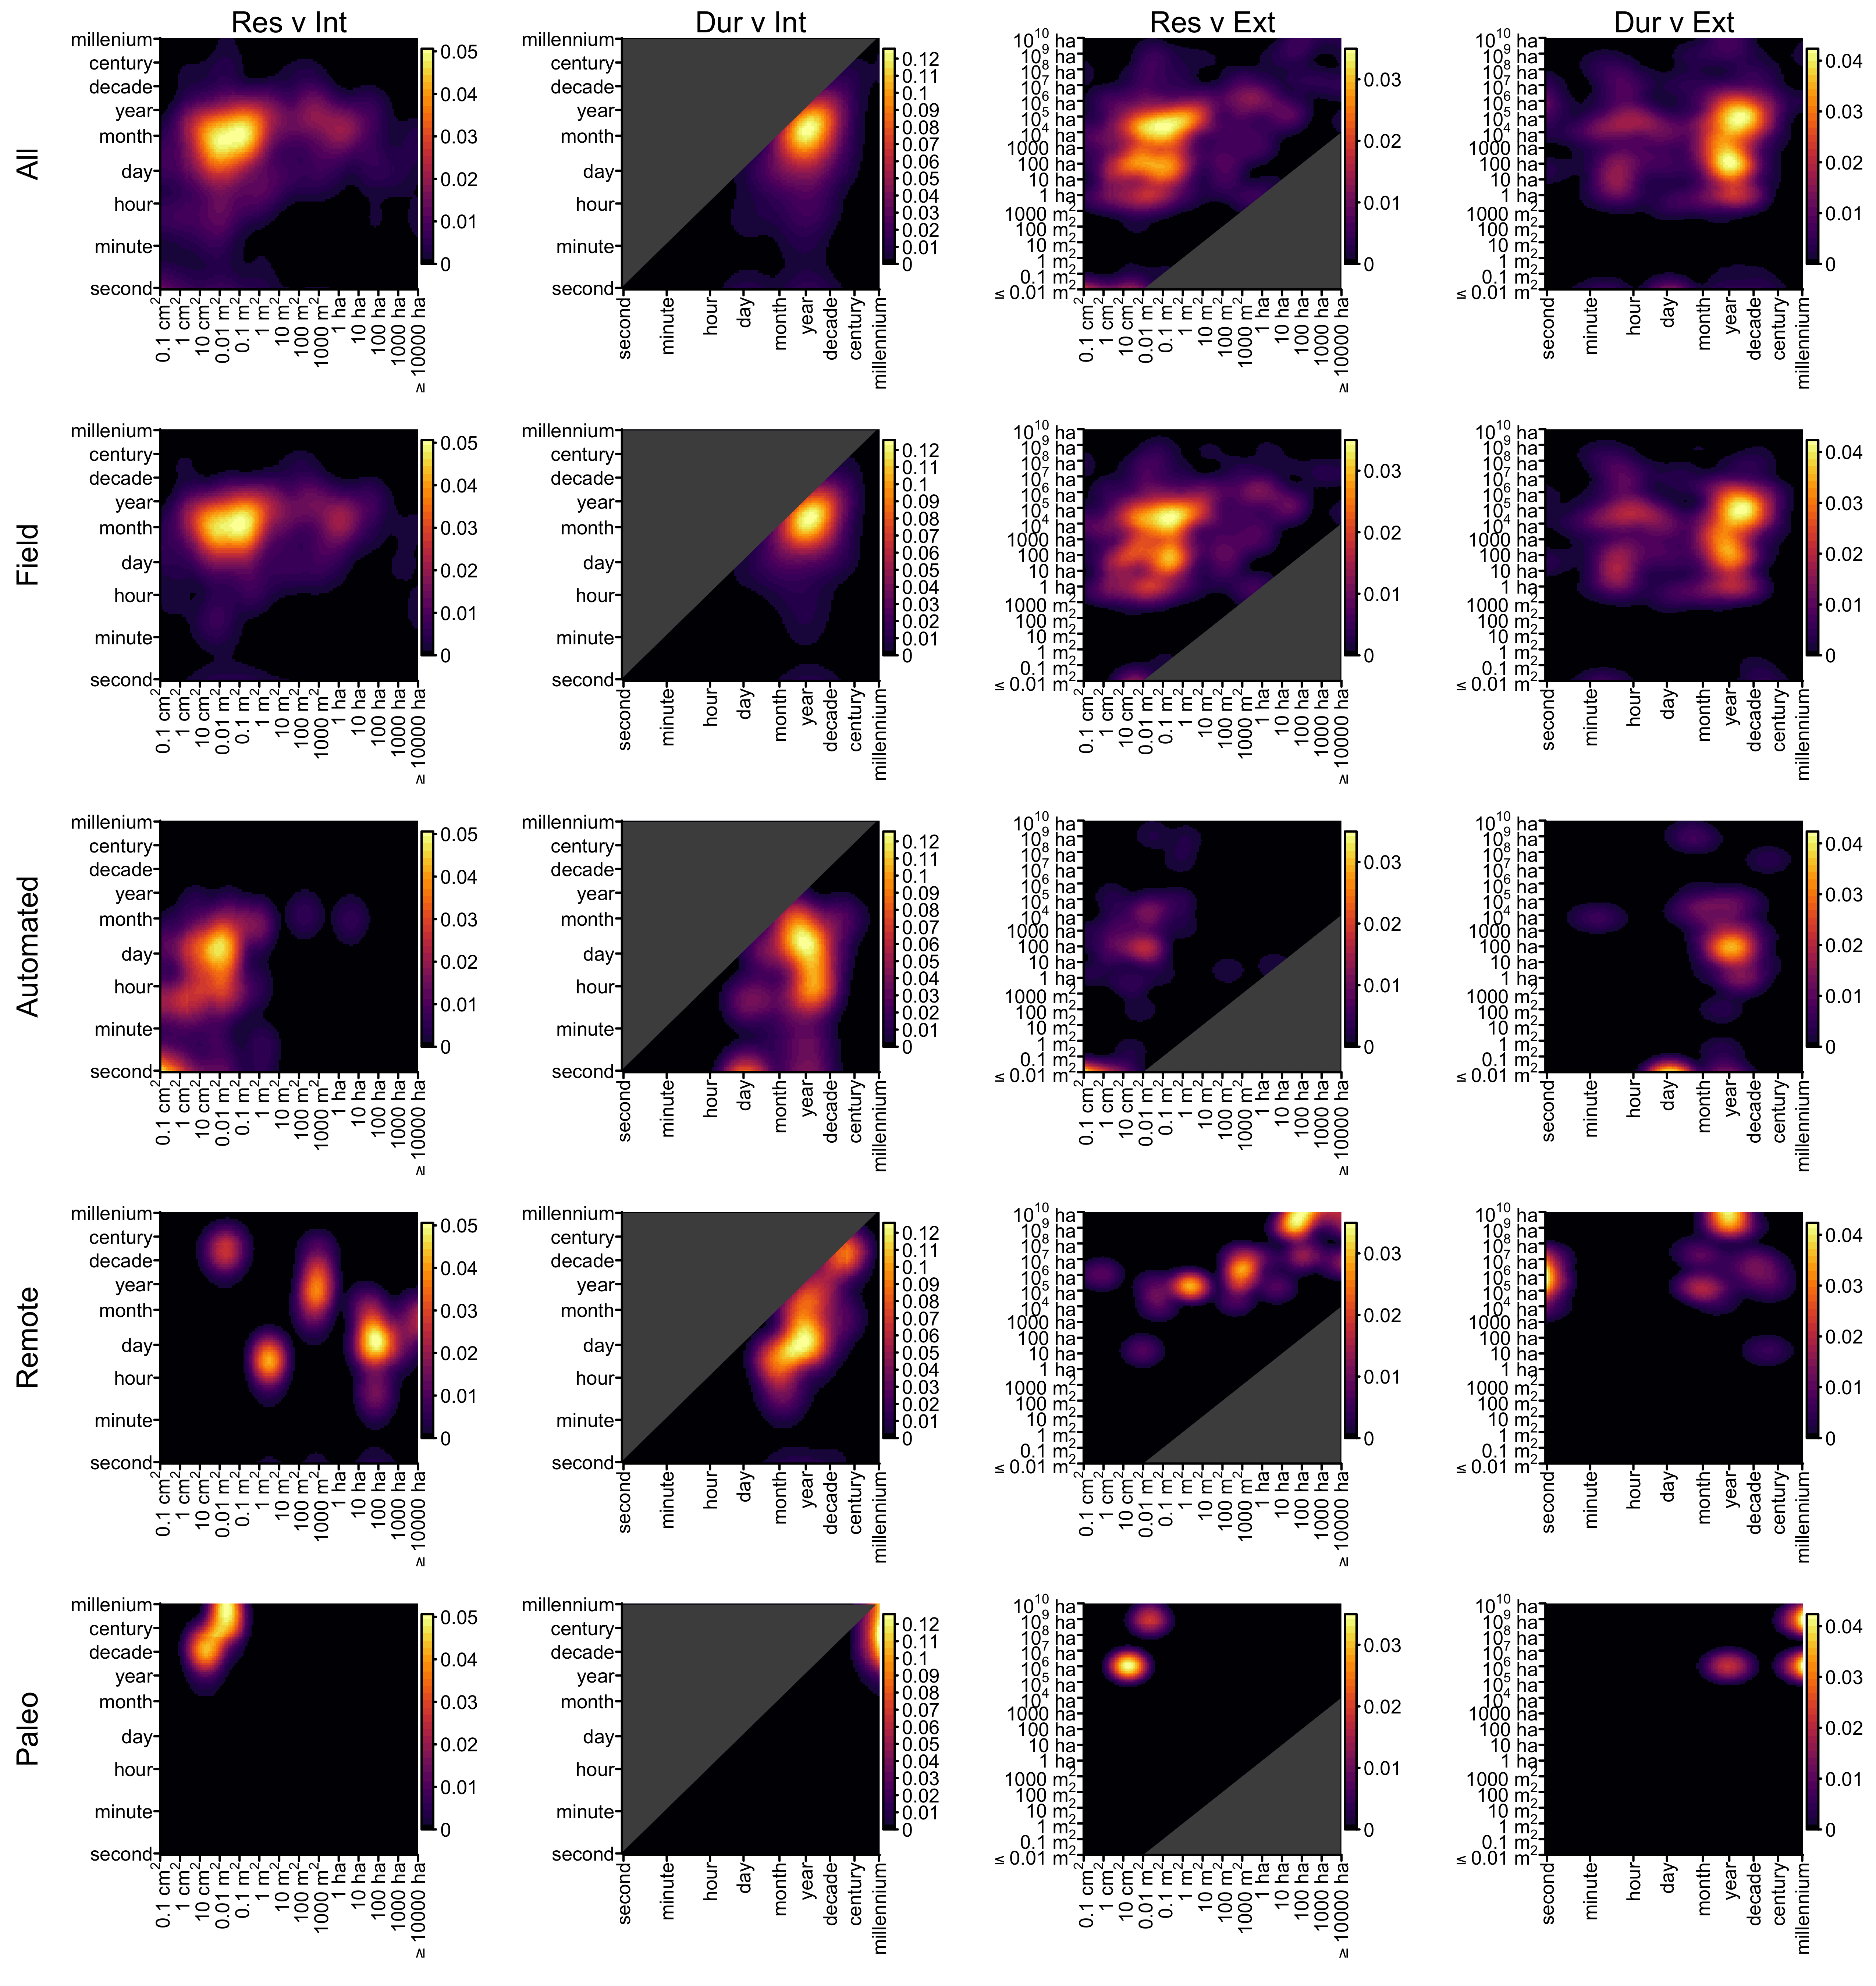
\includegraphics[width=1\textwidth]{../vignettes/figures/figS2.png}
\vspace{-20 pt}
\caption{Kernel density estimates across all observational methods (top row) and for each of the four primary observational methods (rows 2-5). Density estimates for resolution (x axis) versus interval (y axis) are presented in the first column, duration (x) versus interval (y) in the second column, resolution (x) versus extent (y) in the third column, and duration (x) versus extent (y) in the fourth column. Density estimates were applied to the log-transformed values of each observational dimension, and were rescaled to represent percentages. The grey shaded areas represent physically impossible domains (e.g. intervals greater than duration).}
\label{obskde}
\end{figure}

\begin{figure}[!ht]
%\begin{wrapfigure}{c}{1\textwidth}
\centering
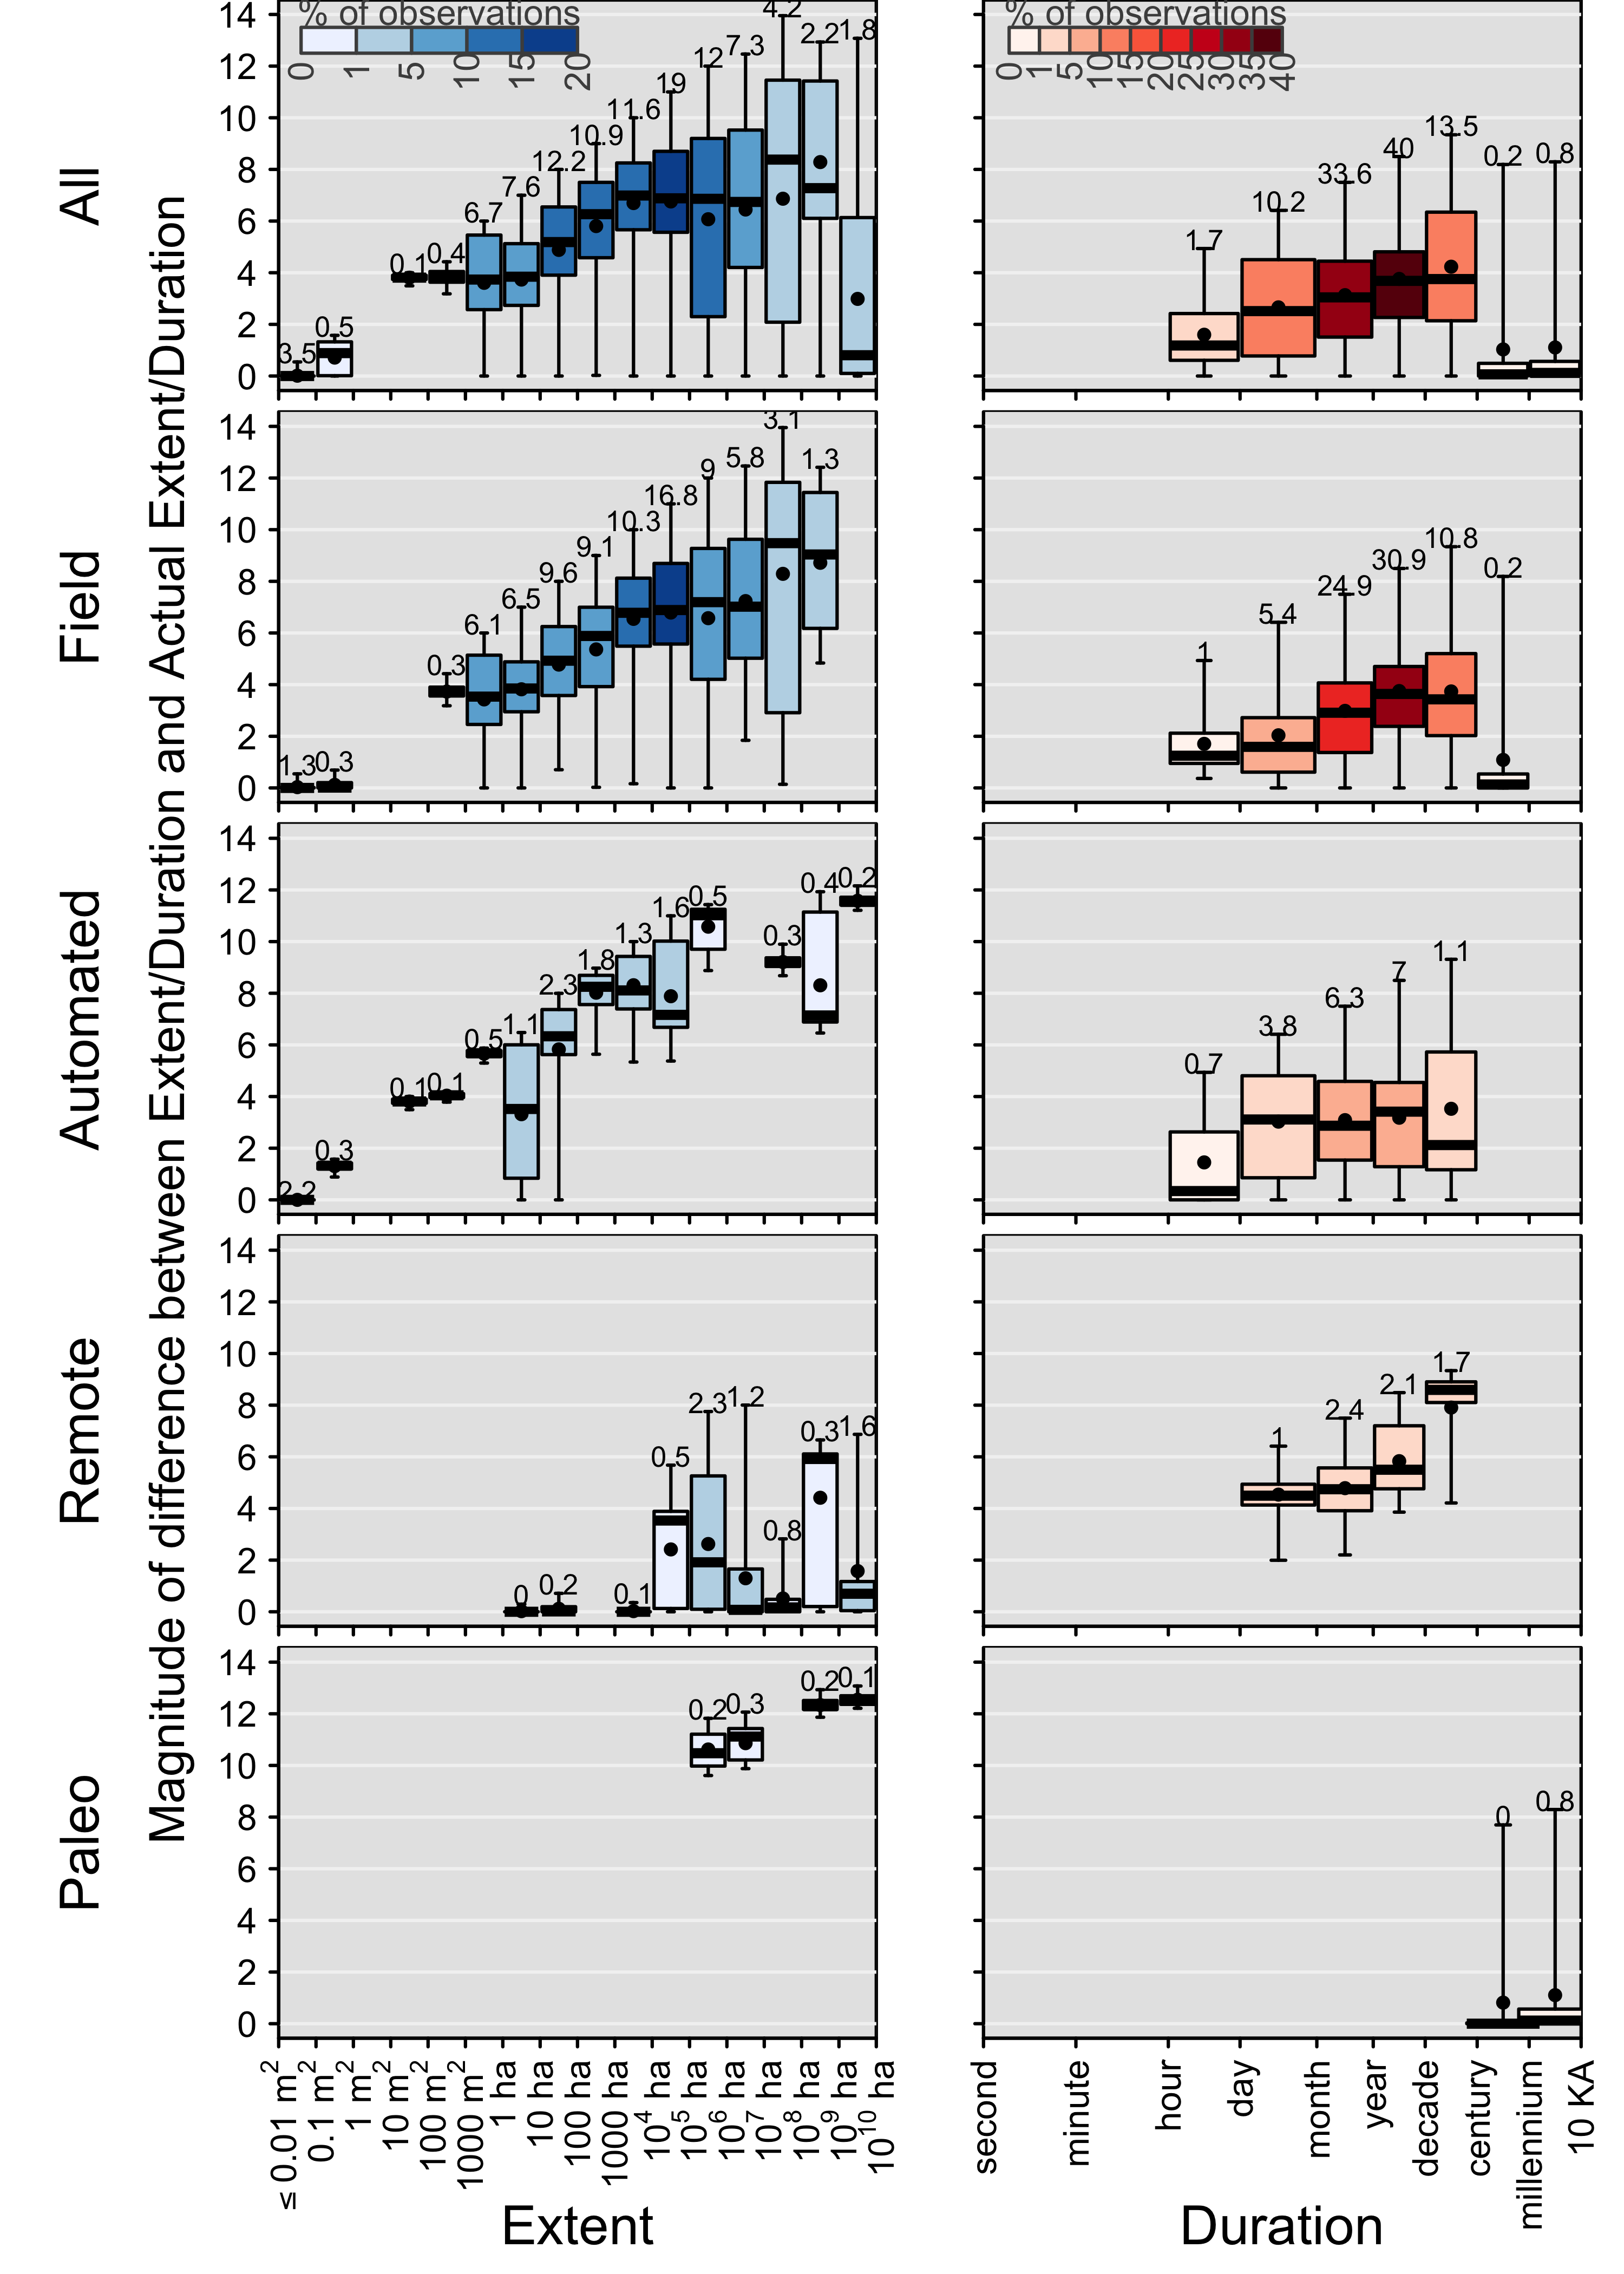
\includegraphics[width=0.7\textwidth]{../vignettes/figures/figS3.png}
\vspace{-5 pt}
\caption{The difference between extent and \emph{actual} extent and duration and \emph{actual} duration, as calculated across all observational methods (top row) and for each of the four primary observational methods. Difference values are expressed in terms of how many orders of magnitude larger (or longer) extent (duration) is than actual extent (actual duration), and are summarized (as box plots, with circle in box representing the mean and line the median) in bins representing increasing scales of actual extent/duration.  The percentages of observations falling within each bin are indicated by the color of the inter-quartile and the numeric value above the upper whisker.}
\label{obsdiff}
\end{figure}

\begin{figure}[!ht]
%\begin{wrapfigure}{c}{1\textwidth}
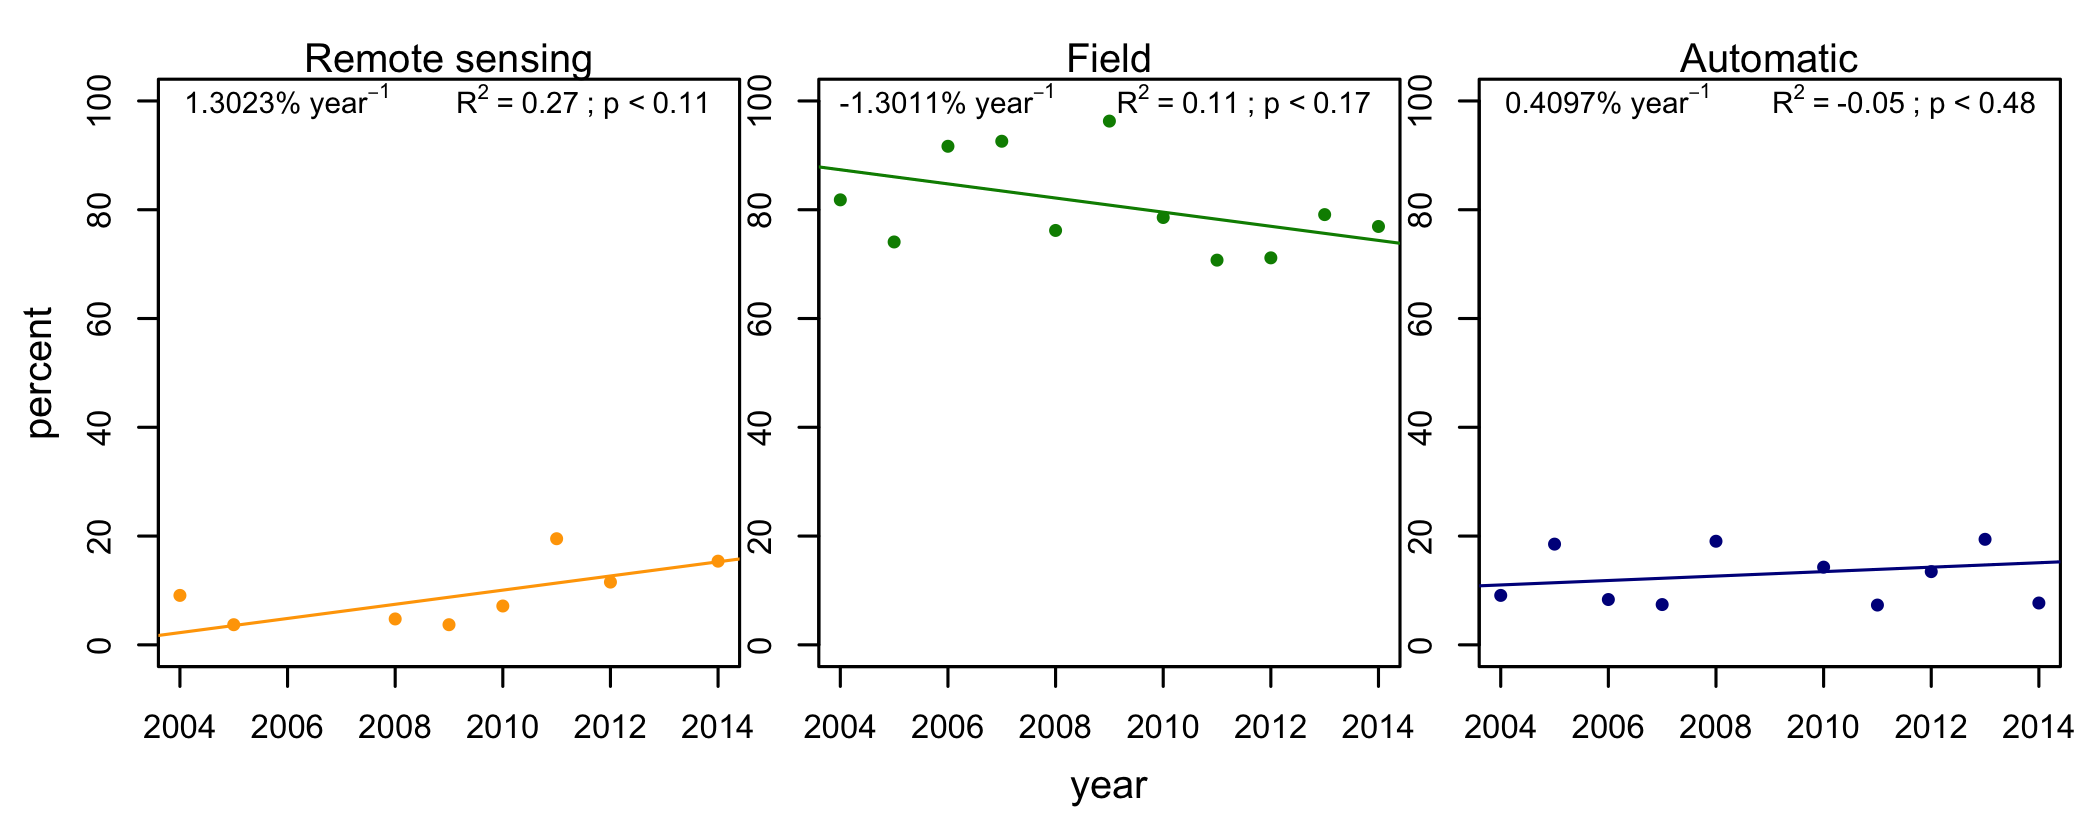
\includegraphics[width=1\textwidth]{../vignettes/figures/figS4.png}
\vspace{10 pt}
\caption{Trends in percentage of observing methods by year of publication. The coefficient of a weighted (by number of studies in each year) linear regression fit to the annual percentages of observations made with remote sensing (left), field methods (center), and automated sensors (right) is presented at the top of each plot, as well as the regression coefficient of determination and p-value. }
\label{type_by_yr}
\end{figure}

\begin{figure}[ht]
%\begin{wrapfigure}{c}{1\textwidth}
\center{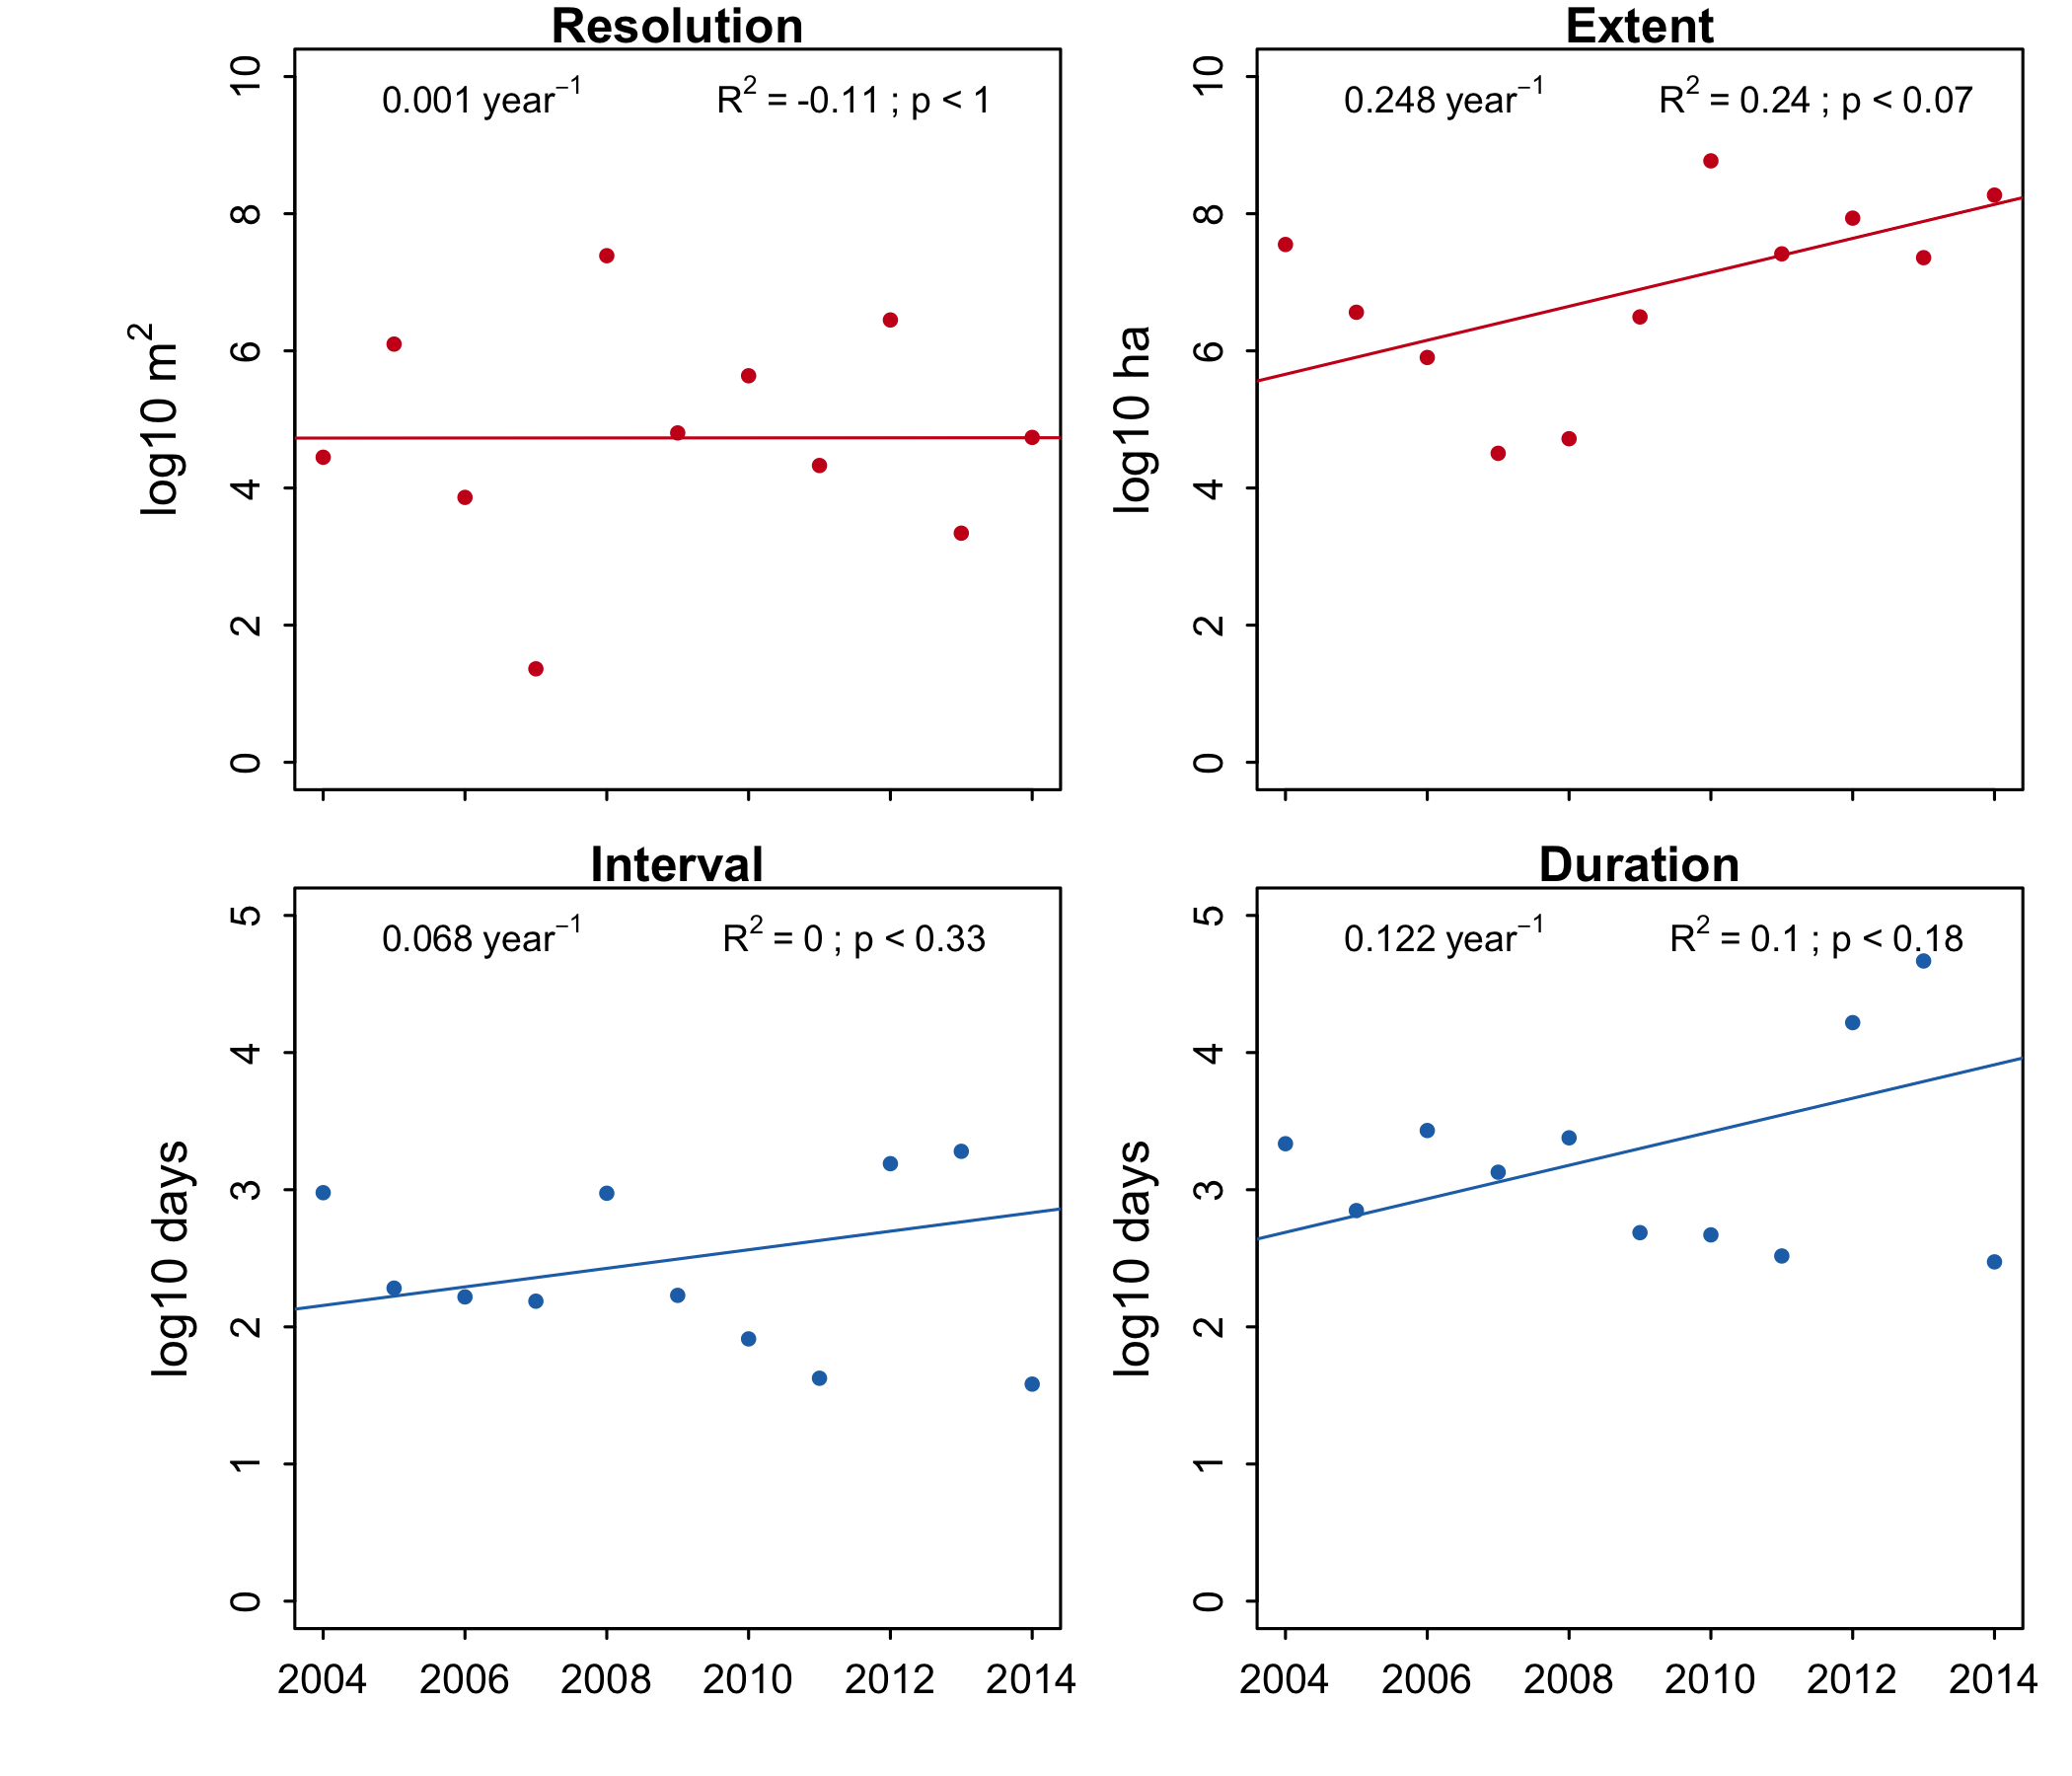
\includegraphics[width=0.8\textwidth]{../vignettes/figures/figS5.png}}
\vspace{5 pt}
\caption{Trends in observational scales by year of publication. The coefficient of a weighted (by number of studies in each year) linear regression, fit to the logarithm (base 10) of the mean scale values (calculated for each publication year) for the six assessed dimensions is presented at the top of each plot, as well as the model coefficient of determination and p-value. }
\label{sc_by_yr}
\end{figure}
%\clearpage

\begin{figure}[!ht]
%\begin{wrapfigure}{c}{1\textwidth}
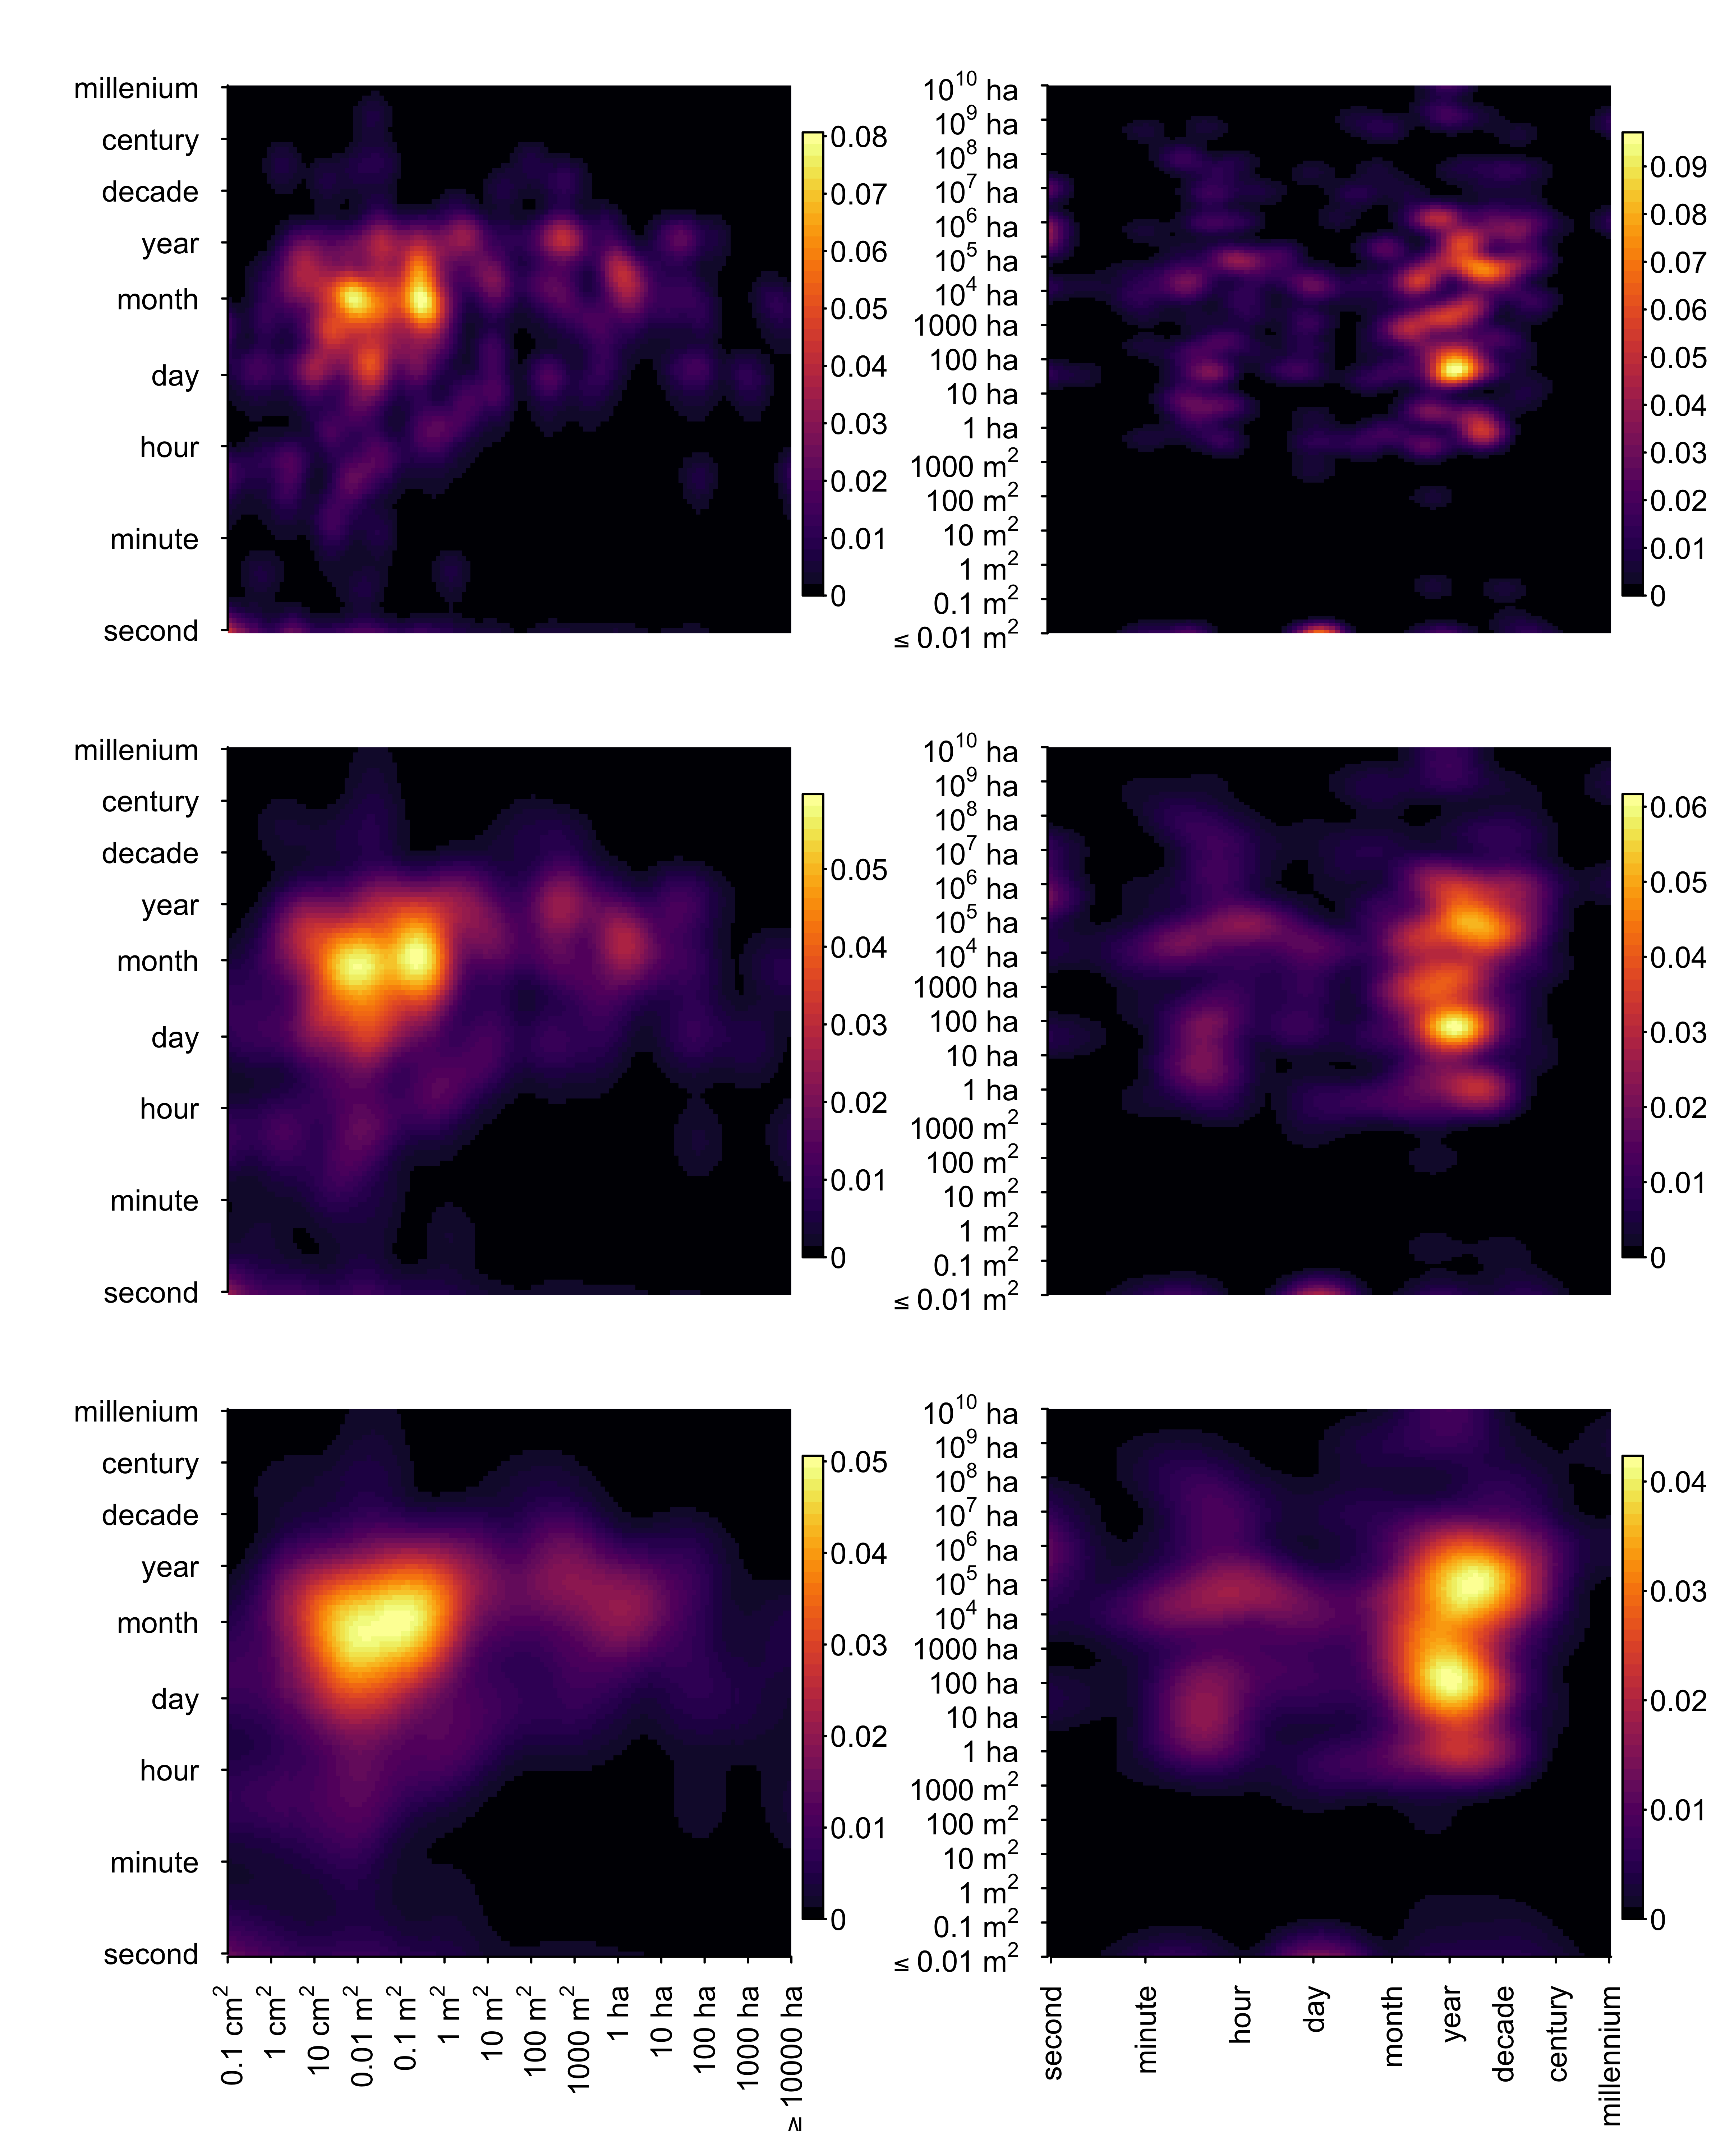
\includegraphics[width=0.9\textwidth]{../vignettes/figures/figS6.png}
\vspace{10 pt}
\caption{Two-dimensional kernel density estimates of observational densities within the domains defined by sampling interval and spatial resolution (left column) and duration and extent (right column), applied to log-transformed values of each observational dimension. Rows indicate the effects of selecting different bandwidths: 0.4 (top row); 0.7 (middle row); 1 (bottom row). }
\label{ksens}
\end{figure}
  
%\subsection*{Rationale}

%\begin{figure}[!ht]
%%\begin{wrapfigure}{c}{1\textwidth}
%\includegraphics[width=1\textwidth]{figures/hists.pdf}
%\vspace{-0.15 cm}
%\caption{Histograms of the spatial resolution (A) and extent (B), sampling interval (C) and temporal duration (D) of ecological observations collected from the surveyed ecological studies. Bars represent percentage of the 367 collected records falling within each bin.}
%\label{afoto1}
%\end{figure}

\clearpage
\bibliography{/Users/lestes/Dropbox/publications/fullbib}

\bibliographystyle{naturemag}

\end{document}




















